\section{Parameter optimization}

We've seen that the results after the simple approach (random choice of the parameter [either usual value or complete random]) can give good result but can also give under expectation ones depending on the method used.

Thus we now try to optimize each parameter used for each methods in order to find the best value to use each time. The data will still kept as it was in the begining.

\subsection{SVM}

On this subsection, the svm will be calculated using the function auto-train and a kfold segmentation of two (one is not accepted) to keep the sample intact and not gives them any advantages.
For the SVM we will use the auto train function given in the Opencv library. As for the stopping point of the algorithm i will use both the max iteration and the epsilon accuracy. But one should keep in mind that this could mean awful result depending on the input since the algorithm tries to approach a maximum and might not reach it as fast as wanted depanding on the start point.

\subsubsection{linear}

The first type of model used was the linear one. The stopping criteria was of either a 100000 iterations (low value to keep consistancy with the following chapter which will require more calculations) or 1 for epsilon.

Results :
\begin{itemize}
  \item Correct classification : 90.08\%;
  \item Wrong classification : 9.92\%;
  \item False positive non ad : 4.82\%;
  \item False positive ad : 5.10\%.
\end{itemize}

The final selected parameter is the following : 0.5 for C. As we can see there is improvement within the results, we go from 81.87\% of correct classification to 90.08\%.

\subsubsection{Polynomial}

For this one, the number of itertion was lowered down to 10000 because the time required for the optimization was too long.

Results :
\begin{itemize}
  \item Correct classification : 93.48\%;
  \item Wrong classification : 6.52\%;
  \item False positive non ad : 5.67\%;
  \item False positive ad : 0.85\%.
\end{itemize}

The optimal parameter selected were :
\begin{itemize}
  \item degree 3.430000;
  \item gamma 0.000010;
  \item ceof0 0.100000;
  \item number of supoport vectors 432.
\end{itemize}

\subsubsection{Radial Basis Function}

We keep 10000 iterations.

Results :
\begin{itemize}
  \item Correct classification : 91.22\%;
  \item Wrong classification : 8.78\%;
  \item False positive non ad : 8.22\%;
  \item False positive ad : 0.57\%.
\end{itemize}

The optimal parameters selected were :
\begin{itemize}
  \item gamma 0.033750;
  \item C 12.500000;
  \item number of supoport vectors 877.
\end{itemize}


\subsubsection{Sigmoid}

Still a 1000 iterations

Results :
\begin{itemize}
  \item Correct classification : 86.4023\%;
  \item Wrong classification : 13.5977\%;
  \item False positive non ad : 6.79887\%;
  \item False positive ad : 6.79887\%.
\end{itemize}

The optimal parameters selected were :
\begin{itemize}
  \item ceof0 0.100000;
  \item gamma 0.000150;
  \item C 0.500000;
  \item number of support vectors 313.
\end{itemize}
Using optimal parameters degree 0.000000, gamma 0.000150, ceof0 0.100000
	 C 0.500000, nu 0.000000, p 0.000000
 Training ...... Done
Number of support vectors for trained SVM = 313


\subsection{Neural Network}

For the neural network, the layers used are as follow :
  \begin{itemize}
    \item input layer, 1558, the number of point in the vector inputs;
    \item output layer, 2 outputs the number of class;
    \item hidden layer, this is the parameter we seek to optimize;
  \end{itemize}

 For this model only the number of cell in the hidden layer will be optimized, not the number of hidden layer (doc here). And the data will be randomized before use. The result shown are with the best parameter each time.

  Results :
  \begin{itemize}
    \item Correct classification : 93.2\%;
    \item Wrong classification : 6.80\%;
    \item False positive non ad : 3.34\%;
    \item False positive ad : 3.34\%.
  \end{itemize}


  \begin{figure}[h]
   \centering
   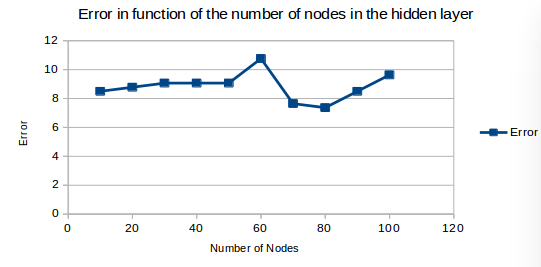
\includegraphics[scale=0.5]{../images/NNPO.png}
   \caption{Class diagram}
  \end{figure}

\subsection{Random forest}
For the random forrest i only played with the following parameter as it's the same with more, only giving more calculations :
  \begin{itemize}
    \item number of variable randomly selected sqrt(n) (usually the best number);
  \end{itemize}
Results :
\begin{itemize}
  \item Correct classification : 95.7507\%;
  \item Wrong classification : 4.24929\%;
  \item False positive non ad : 2.83286\%;
  \item False positive ad : 1.41643\%.
\end{itemize}

\begin{figure}[h]
 \centering
 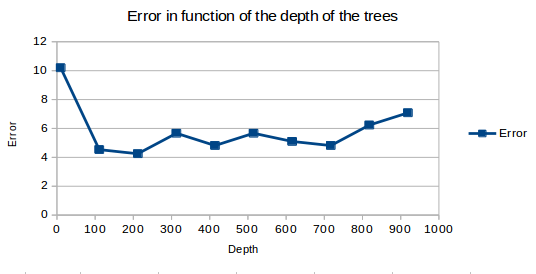
\includegraphics[scale=0.5]{../images/RFPO.png}
 \caption{Class diagram}
\end{figure}
